%
% File acl2017.tex
%
%% Based on the style files for ACL-2015, with some improvements
%%  taken from the NAACL-2016 style
%% Based on the style files for ACL-2014, which were, in turn,
%% based on ACL-2013, ACL-2012, ACL-2011, ACL-2010, ACL-IJCNLP-2009,
%% EACL-2009, IJCNLP-2008...
%% Based on the style files for EACL 2006 by 
%%e.agirre@ehu.es or Sergi.Balari@uab.es
%% and that of ACL 08 by Joakim Nivre and Noah Smith

\documentclass[11pt,a4paper]{article}
\usepackage[hyperref]{acl2017}
\usepackage{times}
\usepackage{latexsym}
\usepackage{footnote}
\usepackage[bottom]{footmisc}
\usepackage{amsmath}

\usepackage{graphicx}
\graphicspath{ {images/} }

\bibliographystyle{acl_natbib}

\usepackage{url}

\aclfinalcopy % Uncomment this line for the final submission
%\def\aclpaperid{***} %  Enter the acl Paper ID here

%\setlength\titlebox{5cm}
% You can expand the titlebox if you need extra space
% to show all the authors. Please do not make the titlebox
% smaller than 5cm (the original size); we will check this
% in the camera-ready version and ask you to change it back.

\newcommand\BibTeX{B{\sc ib}\TeX}

\title{Transliteration as Machine Translation\footnote{This work is done as a part of the author's independent study with Dr. Chris Callison-Burch at University of Pennsylvania.}}

\author{Devanshu Jain \\
  University of Pennsylvania \\
  {\tt devjain@cis.upenn.edu} \\\And
  Chris Callison-Burch \\
  University of Pennsylvania \\
  {\tt ccb@cis.upenn.edu} \\}

\date{}

\begin{document}
\maketitle
\begin{abstract}
Machine Transliteration is the process phonetic translation of a word across different scripts. This is an important and significant task in the field of Natural Language Processing, particularly because of the value it adds to many downstream applications such as Machine Translation, Entity Discovery, Information Retrieval in the context of multilingualism. This is also a difficult task, from the perspective of machine learning especially due to lack of high-quality training data. The objective of this paper is to report the results of many experiments conducted by the authors to improve the results of this task in a low resource environment.
\end{abstract}

\section{Introduction}
Machine Transliteration is the process phonetic translation of a word across different scripts. When a word is translated from its native script to foreign script, then it is called \textit{forward transliteration}. On the other hand, when it is translated from a foreign script back to its native script, then it is called \textit{backward transliteration}.
\par
With growing multilingualism, machine transliteration plays an important role in many downstream applications. One such example is Machine Translation Systems. Almost always, named entities (such as names, addresses, technical terms, festivals, etc.) are transliterated while generating annotated parallel corpora. Sometimes, there are no words in the target language corresponding to a word in the source language. Here, machine transliteration proves to be an important module to improve the performance of machine translation.
\par
Another application is Cross Lingual Information Retrieval (CLIR) Systems. Many of the search engines do not consider transliterated content while responding to a query. It can be observed that the same query (for example, song lyrics) returns significantly different results when submitted to a search engine in a transliterated form. 
\par
An interesting human behaviour is also observed on websites such as Facebook, Twitter, etc. which are sources for a lot of user generated content. A lot of these posts/tweets are written in user's native language transliterated to Roman Script. Machine Transliteration would be a useful component for text-based applications such as Question Answering, Sentiment Analysis, etc.
\par
Machine Transliteration presents its own set of challenges. One of them is of multiple target candidates. For example {hamare} can be written as \textit{humare} or \textit{hamare} or \textit{hamaare} and so on. This leads to the system learning various rules, all of which are correct but may introduce test error. Thus, we need an appropriate performance measure that takes into account the partial correctness of transliteration process. Moreover, there is a lack of high quality training data which hurdles the creation of accurate models.
\par
This study is based on Irvine et.al.'s paper titled "Transliterating From All Languages" (2010). I attempt to recreate some of their experiments with focus on low resource languages to build an end to end machine transliteration system that takes a sequence, its source script and the target script and does the phonetic conversion from the source script to the target script.
\par
The rest of the paper is organised as follows. Section 2 describes some of the related work done in this field. Section 3 describes the tools and data used for this study. Section 4 describes the Baseline System. Section 5 describes the experiments conducted by the authors. Section 6 presents our results and provides some analysis. We have provided some possible future work in section 7.

\section{Related Work}
There are mainly two approaches followed for this task:
\begin{enumerate}
\item Phoneme-Based
\item Grapheme-Based
\end{enumerate}
In Phoneme-Based approaches, the transliteration process is modelled by converting grapheme based representation in source language to source language's phonetic representation to target language's phonetic representation to grapheme based representation in target language. On the other hand, Grapheme-Based approach omits the phonetic representations altogether and maps the source language grapheme to target language grapheme.
\par
\citet*{knight-graehl-1} followed a phoneme-based approach for back-transliterating \textit{Japanese} to \textit{English} and learnt a generative-model using Weighted Finite State Machines. They implemented Dijkstra's shortest path and k-shortest path algorithms to extract the best transliterations. \citet*{virga-khudanpur-1} also followed a phoneme-based approach to transliterate English named-entities to Chinese. They modelled transliteration as a machine translation task and used IBM Noisy Source Channel modelling for the same.
\par
\citet*{kumaran-1} followed a grapheme-based approach to transliterate from English to {Hindi, Tamil, Japanese, Arabic} and vice-versa using IBM Noisy Source Channel modelling. \citet*{ganesh-1} also follows a grapheme based approach but they approach it as a sequence labelling  task. They also used this technique to build a Hindi-English transliteration system. 
\par
Some \citet*{oh-hybrid-1} have also tried to use a hybrid approach using both phoneme and grapheme based approaches for transliteration.
\par
In 2009, Named Entity Workshop (NEWS) introduced a shared task on Machine Transliteration. The latest version (sixth) of the task was held In 2016. The best performing team this year was \citet*{finch-news-2016-1}. They used ensembles of pure neural-network based system. They overcome the general weakness of a unidirectional sequence-to-sequence transducer: error propagation that leads to an output with high-quality prefixes but low-quality suffixes by deploying a bidirectional sequence-to-sequence model that generate from left-to-right and right-to-left. 
\par
Some have also tried to study the transliteration in the context of a low-resource language. \citet*{chinnakotla-1} presented a way to build a transliteration system for low-resource languages i.e., for which large parallel corpora isn't available. They made use of monolingual resources and non-probabilistic manually created character mappings for this purpose. \citet*{kumaran-2} explores compositional transliteration i.e. using an intermediate language Y for transliterating from X $\to$ Y $\to$ Z. This technique claims to improve the system performance parallel corpora is available for language pairs: (X,Y) and (Y,Z) but not for (X,Z).

\section{Base Study}
\citet*{burch-1} paper titled "Transliterating From All Languages" was used as a basis for this study. They treated Machine Transliteration as a monotone character translation task.

\subsection{Tool - Joshua}
\citet{burch-1} used an off the shelf tool called Joshua \citet{li-joshua-1} for their experiments. Joshua is an open source toolkit for Statistical Machine Translation. It provides a scalable, expandable and end-to-end solution for most of the translation tasks. Joshua implements efficient algorithms for Training corpus sub-sampling suffix array grammar extraction, Language Modelling, Decoding Algorithms and parameter tuning. It includes all the components that are required for phrase-based machine translation. To use them, Joshua provides a pipeline perl-script to use these components in different phases: preprocessing the data, creating word alignments, training language models, grammar extraction, tuning, testing and analysis. 
\par
\citet{burch-1} treated transliteration as a phoneme-based monotone character translation task, following \citet*{virga-khudanpur-1}. However, they used log-linear formulation instead of noisy-channel formulation. They used Berkeley aligner for aligning characters in the parallel corpora. Since transliteration is a monotone task, i.e. characters don't need reorganisation within the word, they don't extract the grammar rules that involve any hierarchial structure by restricting the number of non-terminals to 0. They used 10-gram language model. All the data was preprocessed by replacing spaces with underscores('\_') and including spaces between consecutive characters. Special characters were also ended to denote the start and end of words. They used Joshua's MERT optimisation to tune the parameters for their \textit{"translation"} model by optimising the BLEU score objective function. 

\subsection{Data}
\citet{burch-1} used data comprising of named-pairs extracted from Wikipedia articles. Wikipedia maintains pairs of articles written in different languages. They made use of feature that named-entities are mostly transliterated rather than translated from their canonical language to the target language. They mined Wikipedia category pages like: "1961 births" to get a list of people. They made use of such listings and the language links associated with each person to create data consisting of people names in various languages. Data was collected for approximately 200 languages.
\par
Data was further cleaned for use. Some titles were not consistently transliterated. Reasons for this included abbreviations (A.P.J. Abdul Kalam in Roman written as Abul Pakir Jainulabdeen Abdul Kalam in Devanagari). Another reason was that sometimes, middle name was omitted during transliteration i.e. Abbot Suger in Roman was written as Suger in Russian. They computed word-alignments for the data and chose a threshold score for removing the extreme cases of such occurrences.
\par
They also built their own character-based language model for English by tagging and counting named-entities in the English-Gigaword Corpus.

\subsection{Evaluation Metrics}
\citet{burch-1} used Levenshtein distance to evaluate the quality of their transliteration. The distance measures the minimum number of insertions, deletions and substitutions needed to convert the source string to the target string. The distance was normalised by the length of the reference string. The score obtained by averaging the distance over the number of samples in the dataset was used as an evaluation metric for the transliteration system.

\subsection{Experiments and Observations}
\citet{burch-1} experimented with transliterating over 13 languages to English. They performed 10 fold-cross validation using 80\% data for training, 10\% for tuning and the remaining 10\% data for testing. They observed that it was not always true that languages with the largest training corpus gives a better result over the languages with smaller corpus. 
\par
They performed a 2$^{nd}$ experiment in which they measured the system performance with progressively increasing training data for each of the 13 systems. Here, it was observed that the performance always increases although the rate of increase slows down as more and more data is added. 
\par
Another experiment was performed to measure a value of n to maximise the accuracy (exact transliterations) of n-best lists. They observed that not much performance is achieved beyond 10-best list.

\section{Experiments}

\subsection{Tool}
Following \citet{burch-1}, we have used Joshua toolkit for phoneme-based transliteration treating the task as a monotone character based translation. We used 8-gram character based language model for our study. We pre-process the data just like them, however, we omit the inclusion of special characters at the word boundaries. The underscore itself ('\_') should be able to handle the individual words.

\subsection{Data}

\begin{figure*}[!htb]
	\centering
    \begin{minipage}{.5\textwidth}
        \centering
        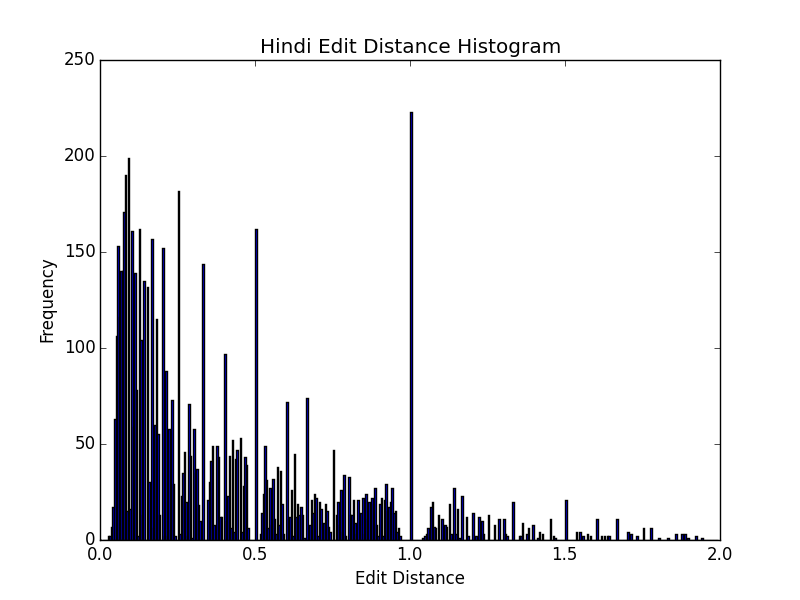
\includegraphics[width=1.0\linewidth]{hi_edit_hist.png}
    \end{minipage}%
    \begin{minipage}{0.5\textwidth}
        \centering
        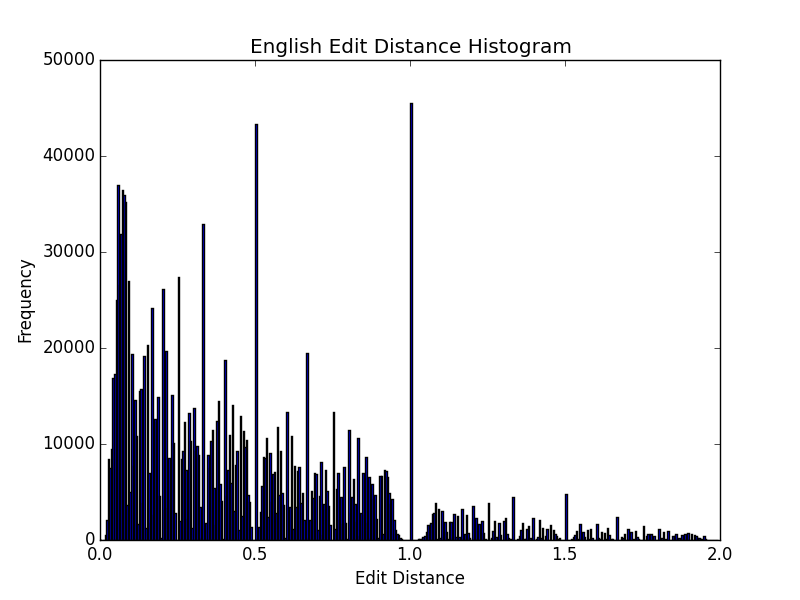
\includegraphics[width=1.0\linewidth]{en_edit_hist.png}
    \end{minipage}
    \caption{Edit distances Histograms}
    \label{fig:edit_hist}
\end{figure*}

We used the same data extracted by \citet{burch-1} using the link given in their paper. In addition, we mined some extra data from Wikipedia to augment it. Wikipedia API provides the service to get backlinks i.e. all the pages that link to a given page. Using this API, we obtain the title of all the pages that link to every a given entity in the original dataset. Using this, we can capture spelling variations for a given named entity. For example, for a page titled "Barack Obama", we obtained pages with titles such as: "Barak Obama", "Barach Obama", "Borrack Obama", "Barack H Obama", "44th President of the United States", etc. Augmenting the original dataset with 1$^{st}$, 2$^{nd}$ and 3$^{rd}$ options seem correct, 4$^{th}$ seems okay but 5$^{th}$ should not be included. To clean the data, we computed a decent threshold for the edit distances between the original page title and backlinked page title. If the edit distance is less than threshold, then the dataset is augmented with the backlinked page title, otherwise not. The threshold was computed empirically by analysing the histograms (Fig. \ref{fig:edit_hist}) of the edit-distances computed as above. We chose a threshold of 0.2 for Hindi Edit Distances and 0.3 for English Edit Distances

\par
\citet{huang-name-origin-1} have shown that having the data corresponding to the word's source of origin may boost transliteration performance. They do it by using a statistical clustering technique to group the data into different classes and then using the transliteration system on each of those classes. To get the named-entity source of origin for our data, we first tried to get the entity's nationality by parsing the original Engish wikipedia article and using regular expression to parse B from "A is a B" (Amitabh Bachhan is an Indian actor) type of structure in the first sentence. We also tried to replicate \citet{huang-name-origin-1} experiment with our dataset and compare the performance for both the techniques. 
\par
For our experiments, we only considered the transliteration from Hindi (Devanagri) to English (Roman). There were around ~10,000 samples for this pair in the original dataset. Using backlinks augmentation, the sampe size increased to 100,000.

\subsection{Experiment 1}
The objective of this experiment was to confirm the hypothesis that with increase in training data, the system performance increases. The Devanagri-Roman data was divided into 3 parts: training, tuning and testing for each such repetition in the following way: For each of the repetition, we held back 60\%, 70\%, 80\% and 90\% data for training and used half of the remaining data for tuning and the remaining half for testing. 

\subsection{Experiment 2}
The objective of this experiment was to observe how the system performance changes when we accumulate training data with languages belonging to same script family For example, Hindi, Sanskrit, Marathi, etc. belong to same family. The hypothesis here was that grouping languages with similar script will significantly increase the training data and if the above hypothesis (Experiment 1) is true, then this should increase the system performance. This experiment was created in the same way as above.

\subsection{Experiment 3}
The objective of this experiment was to observe the changes in system performance when we try compositional transliteration. Given the source language script X and target script Z, we wanted to observe the system performance when an intermediate language is chosen in the process. That is, X $\to$ Y $\to$ Z. The hypothesis here was that the error will accumulate over the two conversions and the system performance should decrease drastically. The experiment for each repetition was created as follows: Some percentage of data for X $\to$ Z was held for testing and the rest of the data along with script Y was used to train 2 different models. We used Arabic as our intermediate language (Y) for this experiment.

\subsection{Experiment 4}
The objective of this experiment was to observe whether the presence of additional information such as the source of origin for a language can affect the system performance. The hypothesis here was that since geographically-distant languages have a very different structure, the variety of structure in the training data may make it hard for the learning algorithm to learn the correct rules. We used simple regular expression to parse wikipedia articles corresponding to the entities in the training data and obtained their nationalities. Thereafter, we divided the training data into 2 parts: those which were Indian and those which were English and then, trained separate models for them.

\section{Results}

\subsection{Performance Measures}
We used the following evaluation metrics to calculate the system performance following \citet{report-news2016-1}. Instead of having a list of reference transliteration in the dataset (which is assumed by \citet{report-news2016-1}), we only have 1 reference transliteration. The evaluation formulae are simplified according to this. Here, N is the number of datapoints. The transliteration system outputs a list of transliterated candidates of length n$_i$ for each word w$_i$. c$_{ij}$ is the j$^{th}$-best transliterated word for word w$_{i}$. r$_i$ is the correct transliteration (reference) for w$_i$
\begin{enumerate}
\item \textbf{Top-1 Word Accuracy: } It measures the proportion of data which produces the correct transliteration (exact matching) as the top transliterated candidate with respect to the reference transliteration.
\begin{align*}
	accuracy_i & = \frac{1}{N}\sum_{i=1}^{N}
							\begin{cases}
								1 & \text{if }r_i = c_{i1}\\
								0 & \text{else}
							\end{cases}
\end{align*}
\item \textbf{Top-1 F-Score: } The F-score is the harmonic mean of Precision and Recall. Precision and Recall is calculated using Edit Distance between the top transliterated candidate and the reference. Following formulae are calculated:
\begin{align*}
	LCS(c,r) & = \frac{1}{2}(|c| + |r| - ED(c,r))
\end{align*}
Here, LCS is Least Common Subsequence and ED is the edit distance. Then,
\begin{align*}
	precision_i & = \frac{LCS(c_{i,1}, r_i)}{|c_{i,1}|} \\
	recall_i & = \frac{LCS(c_{i,1}, r_i)}{|r_{i}|} \\
\end{align*}

\item \textbf{Mean Reciprocal Rank: } It calculates the average of the minimum reciprocal rank of a correct transliteration. This score does not really makes sense for our case since we only have one reference string to compare against. This is because it just turns out to be top-k accuracy measure (if there exists a reference string in the output list).
\begin{align*}
	RR_i & = 
		\begin{cases}
			1 & \text{if }\exists k: r_i = c_{i,k} \\
			0 & \text{else}
		\end{cases}
\end{align*}
\item \textbf{Mean Average Precision: } It calculates the mean of average precision over  all the sources words.
\begin{align*}
	MAP & = \frac{1}{N} \sum_{i=1}^{N} \frac{1}{n_i} (\sum_{k=1}^{n_i}num(i,k))
\end{align*}
Here num(i,k) is the number of correct transliterations in k-best output list with respect to the correct transliteration.

\end{enumerate}
\subsection{Results and Discussion}

\section{Future Work}

\bibliography{acl2017}

\end{document}
